\section{Method}
\label{sec:methodology}

In Figure \ref{fig:Hand_pose}, we provide an overall pipeline of our framework for hand-object pose estimation under interaction. The following details our work.

\subsection{Adaptive Fusion}
\label{sec:adaptive_fusion}

\begin{figure}[h!]
	\centering
	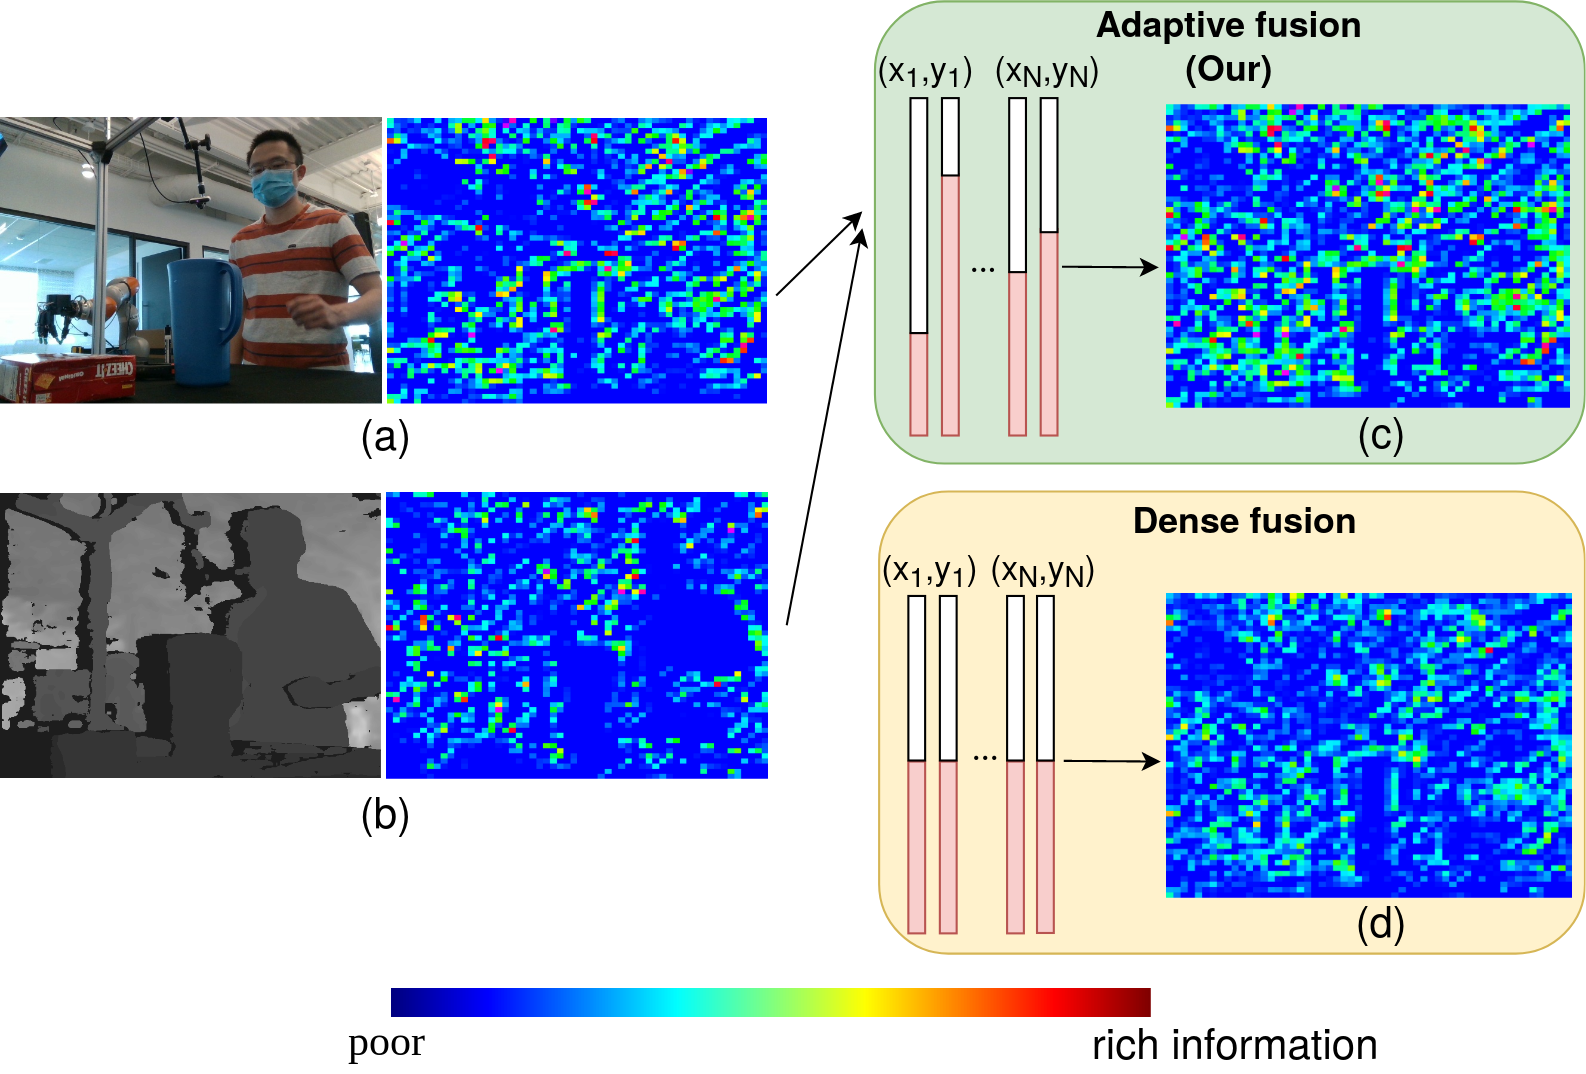
\includegraphics[width=0.95\linewidth]{Figs/Adaptive_fusion.png}
	\caption{\textbf{Adaptive fusion.} Illustration of our proposal adaptive network in comparison with Dense fusion \cite{wang2019densefusion}. The network takes color feature (a) and depth feature (b) as input and learns their diverse distribution of contributing meaningfulness across all positions. Whereas, Dense fusion values RGB and depth feature at each pixel equally. The white and pink columns' height denotes the important degree of each type of feature at each pixel. Intuitively, our output feature (c) is more densely informative than dense fusion output (d).}
	\label{fig:adaptive_fusion}
\end{figure}

Dense fusion \cite{wang2019densefusion} has recently made a remarkable stride in effectively exploiting color and depth images due to two main contributions. The first merit is the capability of extracting geometric features, which conventional RGB-D fusion methods fail to obtain due to applying 2D CNNs for depth images. The second one is introducing pixel-wise fusion to concatenate color and geometric features at a pixel level. However, the network believes 2D and 3D information carried by each pixel are equally valued, while the fact is the opposite. At a specific position, the 2D feature may be remarkable, while the 3D information is latent. To tackle this problem, we propose an adaptive fusion network that learns the favourability distribution of 2D and 3D features for the hand-object pose estimation performance. Figure \ref{fig:adaptive_fusion} illustrates the difference between our work and Dense fusion and presents our more-appealing feature map outcome.

\textbf{Color feature extraction:} Given a color image $I_{rgb} \in \mathbb{R}^{H \times W \times 3}$, the color features $f_{rgb} = \{ f^{rgb}_i \} ^{H \times W}_{i=1}$ are normally extracted by a CNN architecture. Where $f_{rgb} \in \mathbb{R}^{H \times W \times d_{rgb}}$ and each pixel is mapped into a color feature space $f^{rgb}_i \in \mathbb{R}^{d_{rgb}}$. 

\textbf{Depth feature extraction:} The geometric features, on the other hand, are extracted by converting depth maps to point cloud and then feeding into PointNet \cite{qi2017pointnet}. In our work, differing from the original work, we conduct PointNet++ \cite{qi2017pointnet++}, an upgraded version, to replace the original backbone. Given a depth map $I_d \in \mathbb{R}^{H \times W \times 1}$, the point cloud features $f_{geo} = \{f^{geo}_i\}^{H \times W}_{i=1}$.

\textbf{Feature Embedding:} To discriminate the favourability of color and depth features, we add we add learnable weighting matrixes before the fusion process. These matrixes allow each type of feature at each position to be either accelerated or vanished. The output feature is computed as equation \ref{eq:fusion}, where $A$ and $B$ are learnable hyper-parameters. $f^{fusion} \in \mathbb{R}^{H \times W \times (d_{rgb} + d_{geo})}$.


\begin{equation}
	f^{fusion} = A \times f^{rgb} \oplus B \times f^{geo} \
	\label{eq:fusion}
\end{equation}

\subsection{Hand and Object Voting}
\label{sec:voting}
\textbf{Hand joints voting:} As shown in \ref{fig:Hand_pose}, the discriminative features with rich information after the fusion procedure are used to regress hand joints. Conventional voting methods approach object pose estimation including hand poses usually vote for the hand center. Whereas, our method computes votes for hand joints points since hand joints can reflect the hand gestures, which is crucial for hand pose estimation under interaction. The hand joints convey information about the hand shape itself but also the 3D object shape. Therefore, such hand joints are necessary for hand-object interaction learning. We adopt the MANO hand mesh model \cite{romero2022embodied} with 21 hand keypoints $J$ consisting of 16 original hand joints and 5 hand vertices. 

Given the point cloud $\{ p_i \}^{N_{\mathcal{H}}}_{i=1}$ and 21 MANO hand keypoints $\{ Hkp_j \}^{21}_{j=1}$ belong to the same hand $\mathcal{H}$. We denote $p_i = [x_i, f^{fusion}_i]$ with $x_i$ the 3D coordinate and $f^{fusion}_i$ the attentionally fused feature. Similarly, we denote $Hkp_j = [x^{Hkp}_j]$ with $x^{Hkp}_j$ the 3D coordinate of the hand keypoints. We compute the translation offset $\{ {\Delta_{Hkp}}^j_i \}^{21}_{j=1}$ for each point, where ${\Delta_{Hkp}}^j_i$ denotes the translation offset from the $i_{th}$ point to the $j_{th}$ hand keypoint. Thevoted keypoint can be computed as $vHkp^j_i = x_i + {\Delta_{Hkp}}^j_i$. We define the loss for hand keypoints learning as below:
%%%%%%%%%%%%%
\begin{equation}
	\mathcal{L}_{Hkp} = \frac{1}{N_{\mathcal{H}}} \sum_{i=1}^{N_{\mathcal{H}}} \sum_{j=1}^{21} \|{\Delta_{Hkp}}^j_i - {\Delta_{Hkp}}^{j*}_i \|_H \cdot \mathds{1}(p_i \in \mathcal{H}) \
	\label{eq:loss_handjoints}
\end{equation}
%%%%%%%%%%%%%
where ${\Delta_{Hkp}}^{j*}_i$ is the ground truth translation offset, $N_{\mathcal{H}}$ is the total number of points belonging to a hand $\mathcal{H}$. $\| \cdot \|_H$ is the Huber norm. The binary function $\mathds{1}(\cdot)$ equals to 1 when point $p_i$ belongs to a hand $\mathcal{H}$, and 0 otherwise.

\textbf{Object keypoints Selection:} The 3D keypoints are selected from 3D object models. Normally, eight corners of the 3D bounding box are used to represent the object \cite{kong2020sia, doosti2020hope}. However, the corner points are actually far away from points on objects, leading to the difficulty to infer the physical constraints while interacting with the hand. Therefore, we instead select keypoints on the object surfaces that provide ease to learning the hand-object interaction. We use the farthest point sampling (FPS) algorithm to collect the keypoints of objects by initializing an object mesh center point as the first keypoint and then searching the others by FPS until obtaining $M$ keypoints. 

\textbf{Object keypoints voting:} In terms of learning the object presence, the attentionally fused features are fed into a module to predict 3D keypoints for each object. Concretely, given a set of points $\{ p_i \}^{N_{\mathcal{O}}}_{i=1}$ and $M$ selected object keypoints $\{ Okp_j \}^{M}_{j=1}$ belong to the same object $\mathcal{O}$. We denote $Okp_j = [x^{Okp}_j]$ with $x^{Okp}_j$ the 3D coordinate of the object keypoints. The translation offset from the $i_th$ point to the $j_th$ object keypoints is denoted as ${\Delta_{Okp}}^j_i$. Hence, for each point we generate translation offset $\{ {\Delta_{Hkp}}^j_i \}^{M}_{j=1}$. The voted object keypoint can be computed as $vOkp^j_i = x_i + {\Delta_{Okp}}^j_i$. We define the loss function as below:
%%%%%%%%%%%%%%%%%%%%%%%%%%%%%%
\begin{equation}
	\mathcal{L}_{Okp} = \frac{1}{N_{\mathcal{O}}} \sum_{i=1}^{N_{\mathcal{O}}} \sum_{j=1}^{M} \|{\Delta_{Okp}}^j_i - {\Delta_{Okp}}^{j*}_i \|_H \cdot \mathds{1}(p_i \in \mathcal{O}) \
	\label{eq:loss_objectpoints}
\end{equation}
%%%%%%%%%%%%%%%%%%%%%%%%%%%%%%%
where ${\Delta_{Okp}}^{j*}_i$ is the ground truth translation offset, $N_{\mathcal{O}}$ is the total number of points belonging to an object $\mathcal{O}$. $\| \cdot \|_H$ is the Huber norm. The binary function $\mathds{1}(\cdot)$ equals to 1 when point $p_i$ belongs to an object $\mathcal{O}$, and 0 otherwise.

\subsection{Hand and Object Poses Estimation}
\label{sec:interaction}
\begin{figure}[h!]
	\centering
	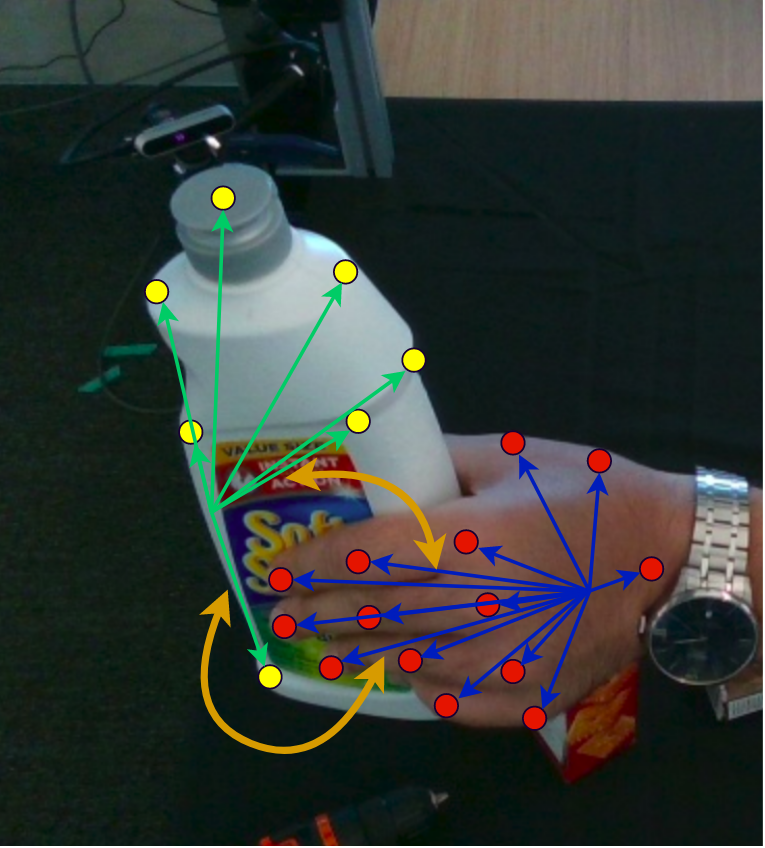
\includegraphics[width=0.6\linewidth]{Figs/Hand-object.png}
	\caption{Illustration of the interaction learning between votes for hand keypoints and votes for object keypoints. The red points denote hand keypoints, while the yellow ones denote object keypoints. The blue and green vectors represent hand keypoints and object keypoints votes, respectively.}
\end{figure}

\textbf{Hand-object interaction learning:} To estimate the hand and object shapes under interactions, voting vectors should be aware of their global neighborhood. Especially, the object keypoints in the vicinity are intuitively beneficial for predicting hand keypoints and vice versa. We adopt a graph convolutional network (GCN) for the interaction learning procedure. Each node of the graph is defined by the proposal position $y_i$ associated with proposal feature $g_i$. In particular, the proposal position is either hand keypoint $(y_i = vHkp^j_i)$ or object keypoint $(y_i = vOkp^j_i)$ and the associated proposal feature $g_i=f^{fusion}_i$. An edge between two nodes is determined by checking the condition of the Euclidean distance between them. If the distance between two neighboring positions $(d_{y_i, y_j} < \delta)$, the edge-feature is defined as:
%%%%%%%%%%%%%%%%%%
\begin{equation}
	e_{ij} = \mathit{h}([y_i,g_i],[y_j, g_j]-[y_j,g_j]) \
	\label{eq:edge_feature}
\end{equation}
%%%%%%%%%%%%%%%%%%%%%%%%%%
where $\mathcal{h}$ is a non-linear fuction. Obtain refined proposal features from intial fusion featues. 

\textbf{Hand and Object pose regression:} we adopt the MANO hand mesh model defined as a manifold triangle mesh $M = (V, F)$ to estimate the final hand pose. $V = \{ v_i \in \mathbb{R}^3 \} \| 1 \leq i \leq n$ is a set of $n=778$ vertices and $F$ is a set of faces. They are parameterized by the MANO parameters $(\theta \in \mathbb{R}^{51}, \beta \in \mathbb{R}^{10})$. We use multi-layer perceptron (MLP) to regress the parameters $(\theta, \beta)$. We define the loss function for hand pose regression as below, where the hand keypoints loss $\mathcal{L}_{Hkp}$ as equation
\ref{eq:loss_handjoints}.
%%%%%%%%%%%%%%%%%%%%%%%%%%%%%%%%%%%
\begin{equation}
	\mathcal{L}_{handpose} = \mathcal{L}_{Hkp} + \mathcal{L}_V + \mathcal{L}_{\theta} + \mathcal{L}_{\beta} \
	\label{eq:loss_handpose}
\end{equation}
%%%%%%%%%%%%%%%%%%%%%%%%%%%%%%%%%%%

In terms of regressing the object pose, we embrace the procedure that maps 6D vectors in representation space produced by the network into the original rotation space and minimizes the differences between the output and the ground-truth rotation matrices. The rigid transformation consists of a rotation $R \in SO(3)$ and a translation $t \in \mathbb{R}^3$. We define the loss function as below:

%%%%%%%%%%%%%%%%%%%%%%%%%%%%%%%%%%%
\begin{equation}
	\mathcal{L}_{objectpose} = \mathcal{L}_{Okp} + \mathcal{L}_t + \mathcal{L}_R	\
	\label{eq:loss_handpose}
\end{equation}
%%%%%%%%%%%%%%%%%%%%%%%%%%%%%%%%%%%

where the loss for object keypoints voting $\mathcal{L}_{Okp}$ is defined as equation \ref{eq:loss_objectpoints}, $\mathcal{L}_t$ is the translation loss. The above rotation loss $\mathcal{L}_R$ is appropriate to asymmetric objects. The rotation metric for symmetric objects is diverse, therefore, given the estimated rotation $\overline{R}$ and translation $\overline{t}$ and the ground-truth $(R^*, t^*)$. The rotation loss is redefined as below:

%%%%%%%%%%%%%%%%%%%%%%%%%%%%%%%%%%%
\begin{equation}
	\mathcal{L}_R = \frac{1}{m} \sum_{x_1 \in \mathcal{M}} \| \min\limits_{x_2 \in \mathcal{M}} (\overline{R}x + \overline{t} - R^*x - t^*) \| \
\end{equation}
%%%%%%%%%%%%%%%%%%%%%%%%%%%%%%%%%%%
where $\mathcal{M}$ denotes the 3D object models and $m$ is the number of points.

Finally, the loss function for hand-object pose estimation under interaction is summarized as below:

\begin{equation}
	\mathcal{L}_{hand-object} = \mathcal{L}_{handpose} + \mathcal{L}_{objectpose} \
	\label{eq:hand-object}
\end{equation}


